\section{Méthode de travail}

\subsection{Méthodologie}

Vu l'envergure du projet et des tâches techniques à accomplir, l'approche sélectionnée pour la réalisation de ce projet est une organisation en mode Agile.
Plus spécifiquement, j'ai décidé de travailler avec le cadre de travail Scrum et son organisation en sprints.

Tout d'abord, j'ai pu définir avec le client les principales fonctionnalités à intégrer dans le projet. Ces fonctionnalités sont classées par ordre de priorité et par temps estimé à la réalisation de celles-ci.

En outre, les principales fonctionnalités contenues dans le projet sont détaillées. S'agissant d'un projet de grande envergure, chacune des principales fonctionnalités a été divisée en petites user stories qui me permettront d'avoir un produit livrable au client à la fin de chaque sprint. Les sprints auront \textbf{une durée d’environ 2 semaines.}

À la fin de chaque sprint, un délivrable correspondant aux tâches / user stories effectuées lors du sprint devra être présenté au client. Ce dernier devra alors vérifier et valider les différentes tâches effectuées.

L'avantage de cette organisation est que, en cas d'erreurs et/ou non validation des tâches de la part du client, ces dernières pourront être revues et corrigées pour le prochain sprint.

\begin{figure}[H]
  \centering
  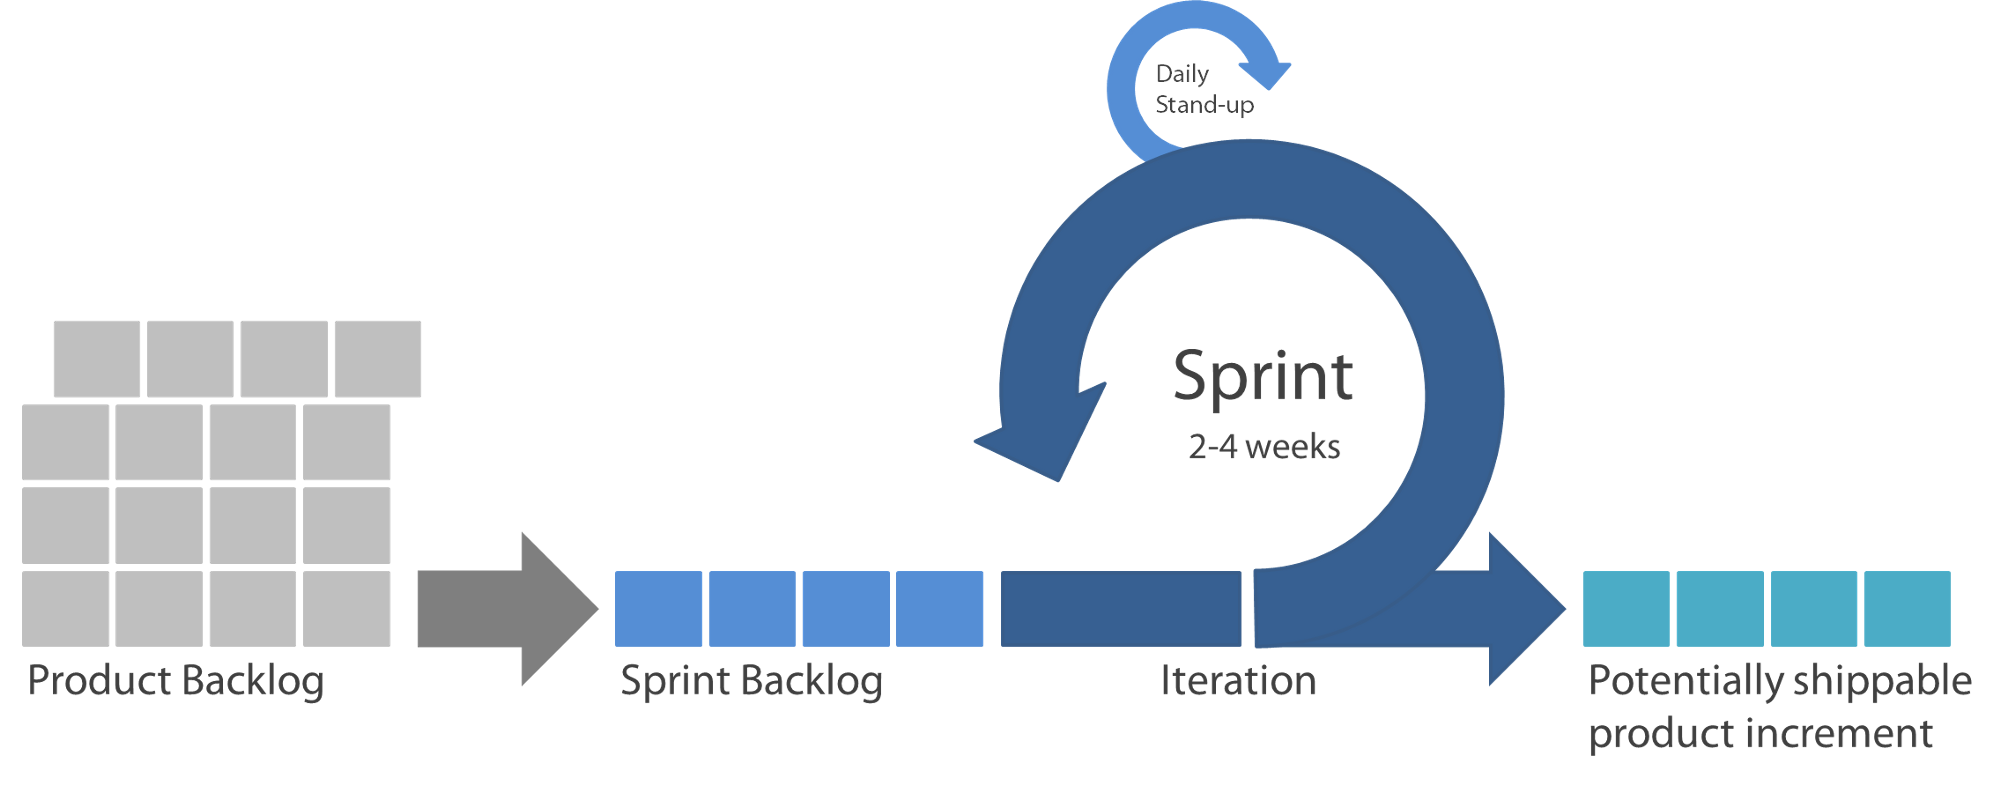
\includegraphics[width=0.75\linewidth]{img/agile.png}
  \caption{ \textit{Cadre de travail Scrum} de Anna Pérez}
  \label{agile}
\end{figure}

\subsubsection{Outils}
Afin d'optimiser les tâches à effectuer pour chaque sprint et d'améliorer ma performance de travail, plusieurs outils ont été utilisés dans l'objectif de faciliter la visualisation de l’avancement du projet.
\begin{itemize}
  \item \textbf{Trello}: Tableau permettant d'organiser les différentes tâches et user stories de manière optimale.
  \item \textbf{Clockify}: Outil de suivi des heures travaillées sur le projet.
  \item \textbf{SqlDBM}: Outil permettant la création de mon schéma de base de données.
\end{itemize}

\subsubsection{Gitflow}

J'ai décidé de travailler avec le gitflow par branche, ce qui permet d'avoir une division au niveau des fonctionnalités qui seront implémentées lors du projet.

\begin{itemize}
  \item Une branche 'develop' qui correspond à la branche 'master' du 'github-flow'
  \item Chaque fonctionnalité est dévéloppée sur une branche spécifique et une fois celle-ci est validée par le client, alors elle est fusionnée avec la branche develop.
\end{itemize}

\begin{figure}[H]
  \centering
  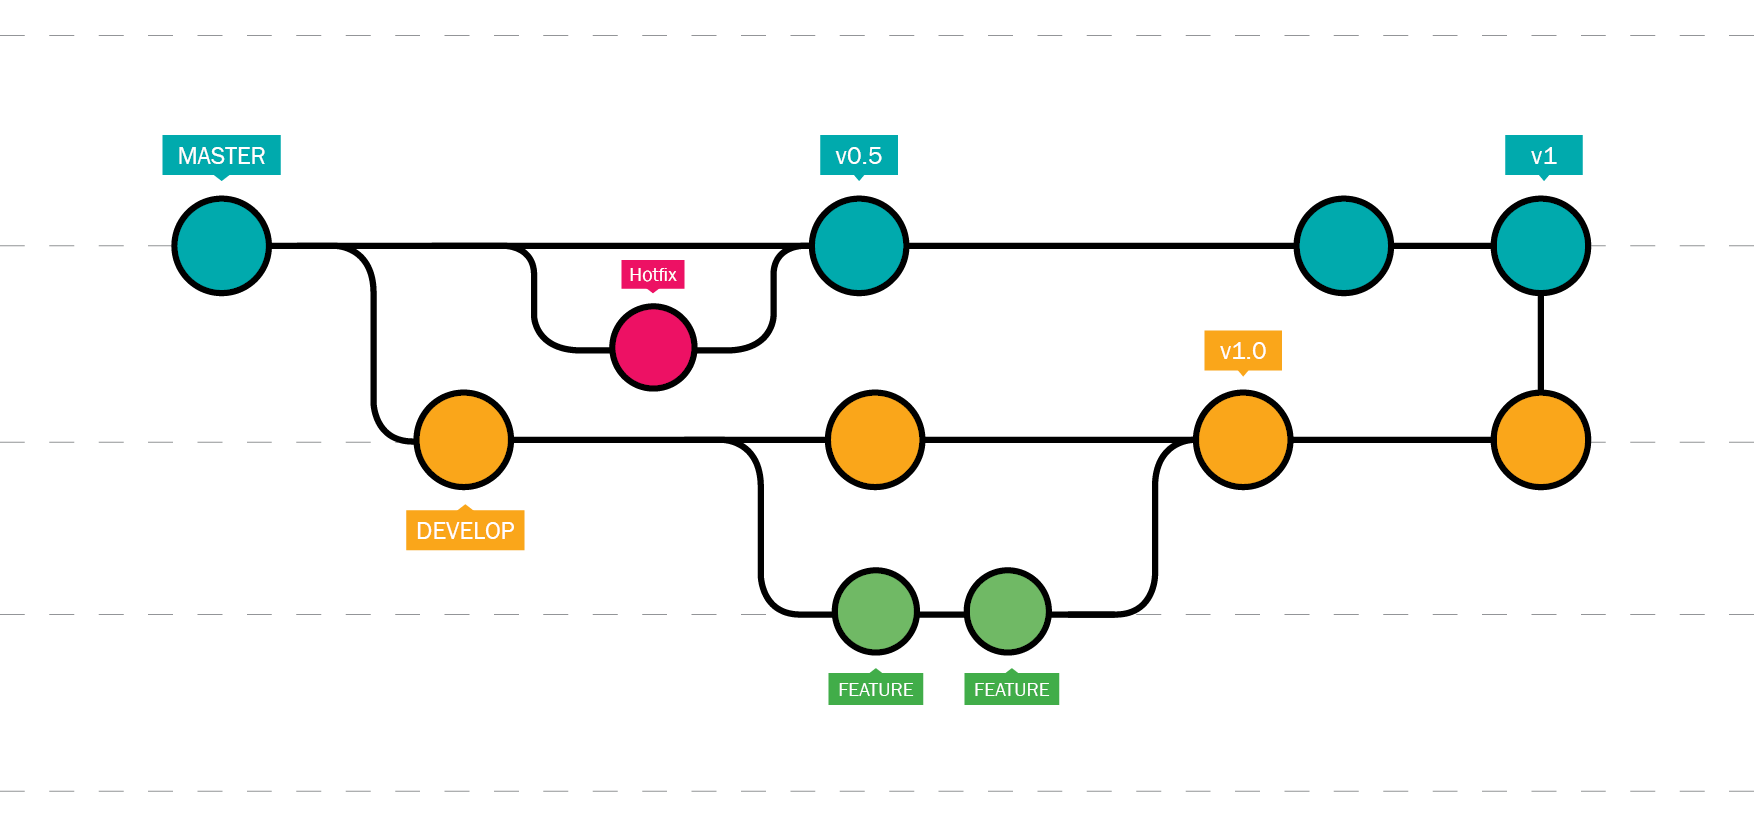
\includegraphics[width=0.75\linewidth]{img/gitflow.png}
  \caption{ \textit{Gitflow Strategy} de Atlassian}
  \label{Gitflow}
\end{figure}


\subsection{Choix des technologies}

\subsubsection{Frontend}
\begin{figure}[H]
  \begin{minipage}{.3\textwidth}
    
\includegraphics[width=0.75\linewidth]{img/react.png}
  \end{minipage}
  \begin{minipage}{.7\textwidth}
    
    En ce qui concerne la technologie frontend, React permet de créer des interfaces utilisateur ou des composants d'interface utilisateur rapides et interactifs pour les utilisateurs d'applications web et mobiles.
    \begin{enumerate}
      \item \textbf{DOM Virtuel}: Il permet de générer le DOM ("Document Object Model", structure des éléments qui sont générés dans le navigateur web lors du chargement d'une page) de manière dynamique, ce qui nous permet de visualiser les changements de données sans devoir recharger à nouveau la page entière, mais seulement le composant qui a été mis à jour.
      \item \textbf{Grande communauté}: Il est soutenu par une large communauté, ce qui nous permet d'avoir un grand nombre de libraires disponibles.
      \item \textbf{Composants réutilisables}: React est constitué de composants qui sont réutilisables, ce qui rend l'application plus portable et plus facile à maintenir.
    \end{enumerate}
    Ces avantages permettent d'améliorer l'expérience de l'utilisateur lors de la navigation dans l'application web, la rapidité du chargement des pages et facilitent la maintenance de l'application.
  \end{minipage}
\end{figure}

\subsubsection{Web Server}

\begin{figure}[H]
  \begin{minipage}{.3\textwidth}
    
\includegraphics[width=0.75\linewidth]{img/caddy.png} 
  \end{minipage} 
  \begin{minipage}{.7\textwidth}
    Au niveau du serveur web, mon choix se porte sur Caddy Server et ce pour plusieurs raisons
    \begin{enumerate}
      \item \textbf{Simple}: Possède une configuration très simple qui nous permettra de le mettre en place en quelques minutes.
      \item \textbf{HTTPS par défaut}: Utilise Let's Encrypt pour mettre le site en HTTPS complet automatiquement, sans aucune configuration et le renouvellement des certificats SSL/TLS se réalise de manière automatique.
      \item \textbf{Multiplateforme}: Il est multiplateforme et je serai en mesure d'exécuter Caddy directement par le biais de Docker, ce qui rendra sa mise en œuvre encore plus facile.
    \end{enumerate}
  \end{minipage} 
\end{figure}

\subsubsection{Backend}
\begin{figure}[H]
  \begin{minipage}{.3\textwidth}
    
\includegraphics[width=0.75\linewidth]{img/node.png} 
  \end{minipage}
  \begin{minipage}{.7\textwidth}

    Comme pour le frontend, le choix du backend est également essentiel. Dans ce cas, j'ai décidé de travailler avec Node.js et ce pour plusieurs raisons.
    \begin{enumerate}
      \item \textbf{Très rapide}: Les tâches courantes comme la lecture ou l’écriture dans la base de données sont exécutées rapidement et il capables de gérer des connexions simultanées à haut débit.
      \item \textbf{Grande communauté}: Il est soutenu par une large communauté, ce qui nous permet d'avoir un grand nombre de libraires disponibles.
      \item \textbf{MVC}: Permet de travailler en MVC, ce qui permet une structure correcte du code.
      \item \textbf{Asynchrone}: Étant un système asynchrone, il permet d’accélérer les applications web. Il est capable d'envoyer gros volumes de données sans bloquer le serveur qui reste ainsi disponible pour traiter d’autres tâches.
      \item \textbf{compatible}: Permet un développement multiplateforme qui est axé sur tous les types d'appareils et de plateformes d'OS (iOS, Android, desktop et web). Le code est réutilisable et entièrement compatible avec tous les principaux systèmes d'exploitation, notamment Linux, Windows, ainsi que macOS, ce qui va nous permettre de rendre notre Web Application accessible depuis toutes les plateformes.
    \end{enumerate}

  \end{minipage}
\end{figure}

\subsubsection{Database}

\begin{figure}[H]
  \begin{minipage}{.3\textwidth}
    
\includegraphics[width=0.75\linewidth]{img/PostgreSql.png} 
  \end{minipage} 
  \begin{minipage}{.7\textwidth}
    Mon choix pour la base de données est PostgreSQL pour plusieurs raisons :
    \begin{enumerate}
      \item \textbf{DB Relationnelle}: Puisque les données doivent être ordonnées et structurées et que des relations doivent exister entre les différentes données, il est essentiel d'utiliser une base de données SQL afin de garantir l'organisation de ces dernières.
      \item \textbf{SQL}: PostgreSQL utilise le langage SQL, qui est le langage le plus utilisé pour les bases de données relationnelles.
      \item \textbf{Compatible}: PostgreSQL est entièrement compatible ACID. ACID est un acronyme pour Atomicité, Cohérence, Isolation et Durabilité. Il garantit donc que les transactions n'interfèrent pas entre elles. Cela garantit les informations contenues dans les bases de données et la pérennité des données dans le système.
      \item \textbf{Hot-Standby}: Il dispose de l'option Hot-Standby qui permet aux utilisateurs d'accéder aux tables en mode lecture pendant que les processus de sauvegarde ou de maintenance sont en cours.

    \end{enumerate}
    PostgreSQL jouit d'une solide réputation en matière de fiabilité, de robustesse des fonctionnalités et des performances.
  \end{minipage} 
\end{figure}


  
\subsection{Autres}
\subsubsection{Documentation API}


L'API (\textit{Application Programming Interfaces}) est le backbone\footnote{\textit{Élement structurelle indispendsable au bon fonctionnement de l'application. Ceci répresente le coeur de l'application.}} d'une application. Elle permet l'interaction d'un utilisateur ou d'une application avec le système d'information sur base d'endpoints.
Pour pouvoir utiliser l'API de manière efficace, il est nécessaire d'avoir une bonne documentation. Cette documentation doit pouvoir exprimé de manière claire l'action de chaque endpoint sur le système d'information. Dès lors on y retrouvera les méthodes telles que GET, CREATE, UPDATE, DELETE, les informations rélatives aux données nécessaires pour le bon déroulement de la requête ainsi qu'un exemple et/ou le format du résultat attendu.
\newpage
Pour pouvoir réaliser cette documentation, il existe un grand nombre de technologies qui permettent de la créer et de la générer automatiquement. Dans mon cas, j'ai décidé d'utiliser \textbf{Swagger}. Celui-ci s'intègre parfaitement avec NodeJS / ExpressJS, il permet d'autogénerer en grande partie la documentation sur base de mes endpoints et il est open-source.
La documentation générée par Swagger est facile à comprendre et permet de tester directement l'API sans devoir passée par un outil supplémentaire tel que Postman.

\begin{figure}[H]
  \centering
  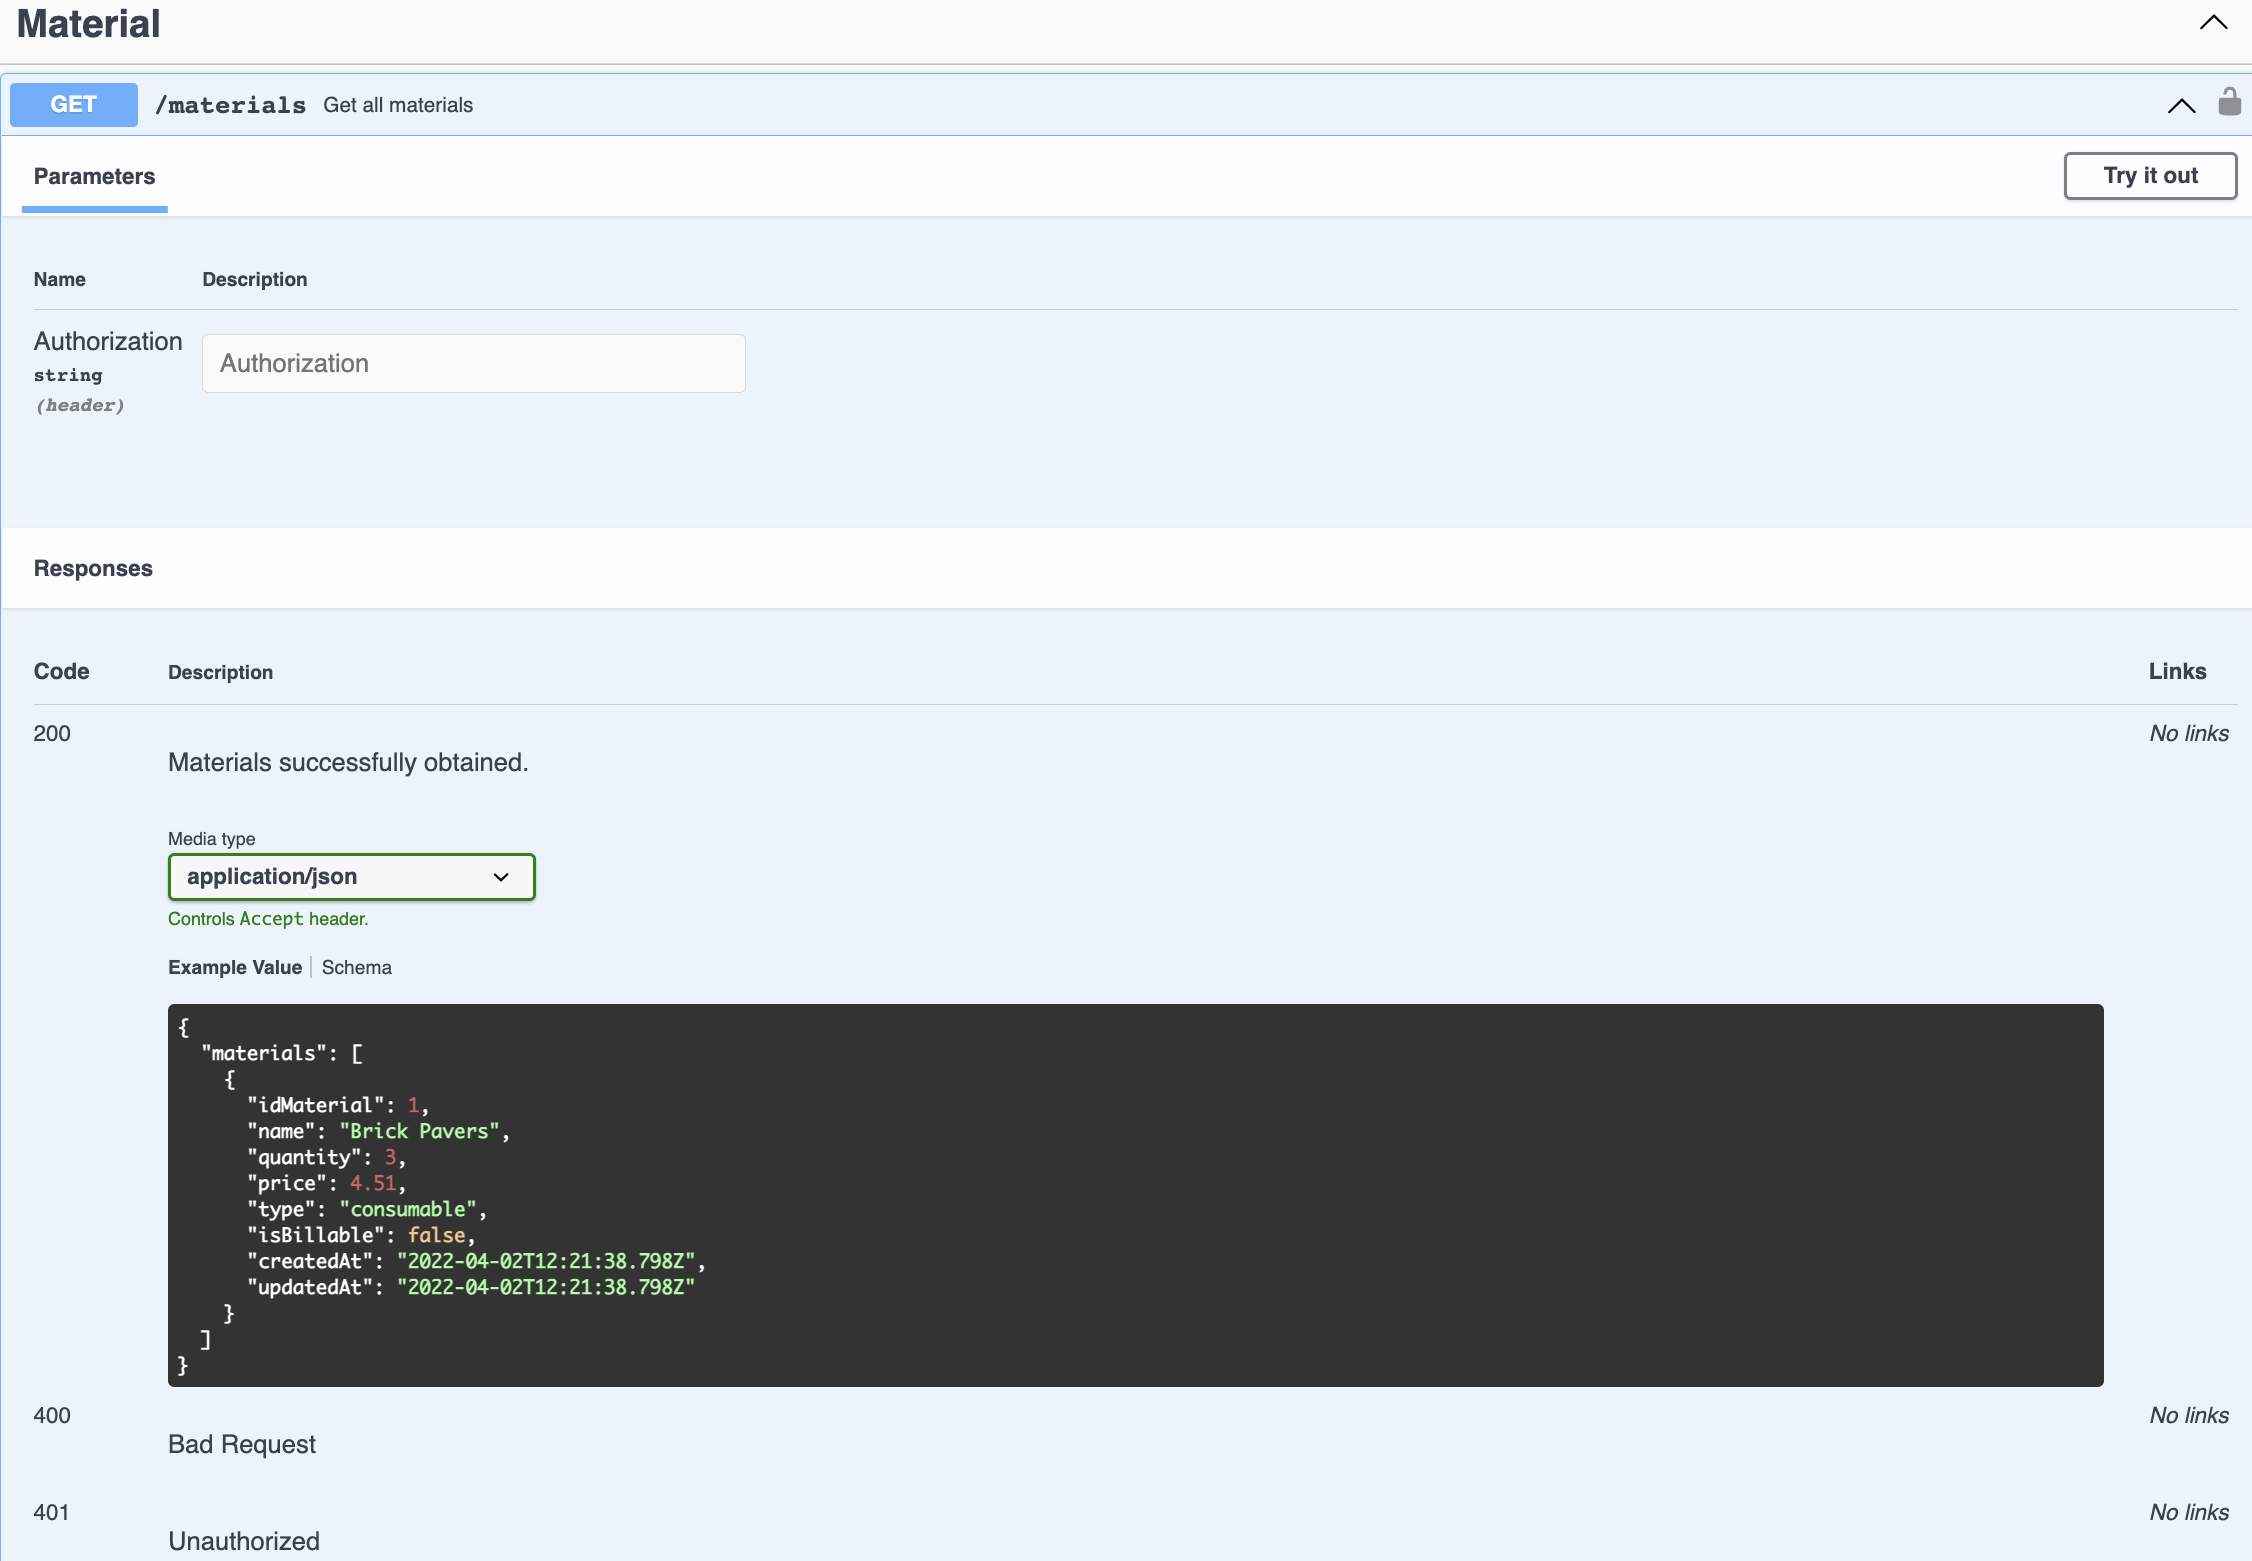
\includegraphics[width=0.75\linewidth]{img/docApi.png}
  \caption{ Documentation API avec Swagger}
  \label{Swagger}
\end{figure}
\subsubsection{Linter}
Dans tout projet, il est inévitable d'avoir des erreurs de syntaxe, des styles de code et bien d'autres problèmes. De plus, avoir un code parfaitement cohérent et lisible est très compliqué. C'est pourquoi l'une des solutions est l'utilisation d'un Linter. Cet outil effectue un check du code source de l'application sans jamais l'exécuter.

Une fois la révision terminée, le Linter nous montre les erreurs de syntaxe, corrige automatiquement l'indentation si cette option a été configurée et fait également des suggestions visant à améliorer le code.

Considérant que c'est une partie essentielle de mon projet, j'ai décidé d'utiliser le Linter et plus précisément ESLint.

